% This file was converted to LaTeX by Writer2LaTeX ver. 1.0.2
% see http://writer2latex.sourceforge.net for more info
\documentclass[a4paper]{article}
\usepackage[utf8]{inputenc}
\usepackage[T3,T1]{fontenc}
\usepackage[slovene,english,french]{babel}
\usepackage[noenc]{tipa}
\usepackage{tipx}
\usepackage[geometry,weather,misc,clock]{ifsym}
\usepackage{pifont}
\usepackage{eurosym}
\usepackage{amsmath}
\usepackage{wasysym}
\usepackage{amssymb,amsfonts,textcomp}
\usepackage{color}
\usepackage{array}
\usepackage{supertabular}
\usepackage{hhline}
\usepackage{hyperref}
\hypersetup{pdftex, colorlinks=true, linkcolor=blue, citecolor=blue, filecolor=blue, urlcolor=blue, pdftitle=Trinity College Dublin, pdfauthor=jacob, pdfsubject=, pdfkeywords=}
\usepackage[pdftex]{graphicx}
% Text styles
\newcommand\textstyletablecaptionCar[1]{\foreignlanguage{english}{\textbf{#1}}}
% Outline numbering
\setcounter{secnumdepth}{2}
\renewcommand\thesection{\arabic{section}}
\renewcommand\thesubsection{\arabic{section}.\arabic{subsection}}
\makeatletter
\newcommand\arraybslash{\let\\\@arraycr}
\makeatother
% List styles
\newcommand\liststyleWWNumvi{%
\renewcommand\theenumi{\arabic{enumi}}
\renewcommand\theenumii{\arabic{enumii}}
\renewcommand\theenumiii{\arabic{enumiii}}
\renewcommand\labelitemi{[F0B7?]}
\renewcommand\labelenumi{\theenumi.}
\renewcommand\labelenumii{\theenumii.}
\renewcommand\labelenumiii{\theenumiii.}
}
% Page layout (geometry)
\setlength\voffset{-1in}
\setlength\hoffset{-1in}
\setlength\topmargin{2.501cm}
\setlength\oddsidemargin{2.501cm}
\setlength\textheight{24.698002cm}
\setlength\textwidth{15.999001cm}
\setlength\footskip{0.0cm}
\setlength\headheight{0cm}
\setlength\headsep{0cm}
% Footnote rule
\setlength{\skip\footins}{0.119cm}
\renewcommand\footnoterule{\vspace*{-0.018cm}\setlength\leftskip{0pt}\setlength\rightskip{0pt plus 1fil}\noindent\textcolor{black}{\rule{0.25\columnwidth}{0.018cm}}\vspace*{0.101cm}}
% Pages styles
\makeatletter
\newcommand\ps@Standard{
  \renewcommand\@oddhead{}
  \renewcommand\@evenhead{}
  \renewcommand\@oddfoot{}
  \renewcommand\@evenfoot{}
  \renewcommand\thepage{\arabic{page}}
}
\makeatother
\pagestyle{Standard}
\setlength\tabcolsep{1mm}
\renewcommand\arraystretch{1.3}
% footnotes configuration
\makeatletter
\renewcommand\thefootnote{\arabic{footnote}}
\makeatother
\title{Trinity College Dublin}
\author{jacob}
\date{2016-02-14}
\begin{document}
\clearpage\setcounter{page}{1}\pagestyle{Standard}
{\centering\selectlanguage{english}\bfseries
INSTRUCTIONS FOR PREPARATION AND SUBMISSION \newline
OF PRINT-READY PAPERS (see last page for more than 2 authors)
\par}


\bigskip

\begin{flushleft}
\tablehead{}
\begin{supertabular}{m{3.8749998cm}m{3.8760002cm}m{3.8760002cm}m{3.8749998cm}}
\selectlanguage{english} Graduate of Trinity College Dublin, 1992.
Completed a masters degree in 1994 on the development of Bridge WIM
systems. Currently director of information research at IMOXIN Data
Plc.. &


\includegraphics[width=2.619cm,height=3.307cm]{openwim-img/openwim-img1.png}
 &


\includegraphics[width=2.619cm,height=3.307cm]{openwim-img/openwim-img2.png}
 &
\selectlanguage{english} Obtained B.E. and M.Sc. from University College
Galway, Ireland and Ph.D. from University of Michigan. Joined WIM data
group in World Data Systems in 1994 where he is an Engineering Systems
Controller.\\
\multicolumn{2}{m{7.951cm}}{\centering
{\selectlanguage{english}\bfseries John W. SMITH}\par

\centering {\selectlanguage{english} University of Cork}\par

\centering \selectlanguage{english} Ireland} &
\multicolumn{2}{m{7.951cm}}{\centering
{\selectlanguage{english}\bfseries Pierre BLANC}\par

\centering {\selectlanguage{english} National Cyrilic Authority of
Wales}\par

\centering \selectlanguage{english} United Kingdom}\\
\end{supertabular}
\end{flushleft}

\bigskip


\bigskip

{\selectlanguage{english}\bfseries
Abstract}

{\selectlanguage{english}
This paper gives instructions for the preparation of papers to be
presented at the 7\textsuperscript{th} International Conference on
Weigh-In-Motion (ICWIM7). It is presented, as far as is possible, in a
style consistent with a conference paper. Abstracts for these papers
should not exceed 10 lines in length. The abstract should be provided
in English and in one other language among French, Portuguese or
Spanish\footnote{ The French, Portuguese or Spanish version will be
edited if needed by a native speaking Scientific Committee member.}.
Nothing except the author details, photographs and abstracts should be
present on the first page.}


\bigskip

{\selectlanguage{english}
The papers will be first published in the conference proceedings, later
on the ISWIM website, and the best ones may be submitted to a Journal
with the authors’ agreement.}


\bigskip

{\selectlanguage{english}
\textstyletablecaptionCar{Keywords:} \ Language, Font, Photograph, Heavy
Vehicles, Freight transport, Weigh-in-Motion, WIM.}


\bigskip

{\selectlanguage{english}\bfseries
\foreignlanguage{french}{Résumé}}

{\selectlanguage{english}
\foreignlanguage{french}{Ce papier donne les instructions pour la
préparation des articles qui seront présentés à la
7}\foreignlanguage{french}{\textsuperscript{e}}\foreignlanguage{french}{
conférence internationale sur le pesage en marche (ICWIM7). Ces
instructions sont aussi proches que possible de celles de la plupart
des articles de conférences. Les résumés de ces articles ne doivent pas
dépasser 10 lignes. Le résumé doit être produit en anglais et dans une
autre langue à choisir parmi le français, l’espagnol ou le portugais.
Rien d’autre que les informations concernant les auteurs, leurs photos
et le résumé ne doit figurer sur la première page.}}


\bigskip

{\selectlanguage{english}
\foreignlanguage{french}{Les articles seront d’abord publiés dans les
actes de la conférence, puis sur le site ISWIM. Les meilleurs pourront
être soumis à une revue avec l’accord des auteurs.}}


\bigskip

{\selectlanguage{english}
\textstyletablecaptionCar{\foreignlanguage{french}{Mots-clés:}}\foreignlanguage{french}{
Langue, police, photos, poids lourds, transport de marchandises, pesage
en marche, WIM.}}

\section{Paper Parts}
{\selectlanguage{english}
Each paper should have the following parts:}

\liststyleWWNumvi
\begin{itemize}
\item {\selectlanguage{english}
title}
\item {\selectlanguage{english}
author(s) information, including photo(s)}
\item {\selectlanguage{english}
abstract in English and second language (French, Portuguese or Spanish,
to be edited by an ISC member)}
\item {\selectlanguage{english}
body of the paper, including any tables and/or figures}
\item {\selectlanguage{english}
list of references.}
\end{itemize}
\section{General Instructions}
{\selectlanguage{english}
Provide papers in electronic form (\textbf{.RTF, .DOC or .DOCX file
required}) with any images placed within the text. The papers will be
published, with no editing other than the author’s on the ISWIM web
site, and in the conference proceedings. Papers not prepared to the
correct presentation standard may be rejected regardless of their
technical content. The editor reserves the right to make minor
editorial changes without consultation with the authors.}

\subsection{Length}
{\selectlanguage{english}
The papers (including title/abstract and reference list pages) must not
exceed 10 pages. Short papers of 6 pages maximum are also welcome for
on-going research or specific topics.}

\subsection{Language }
{\selectlanguage{english}
All papers must be submitted for assessment in English. Authors from
French, Portuguese and Spanish speaking countries and those who may get
translations are encouraged to also submit their final papers (after
revisions) in another language. Such papers will be reviewed and
published on the ISWIM web site, and the best ones may be submitted to
a French, Portuguese or Spanish journal with the authors’ agreement.}

\subsection{Document Style}
{\selectlanguage{english}
Authors are encouraged to use this file of instructions as a template
document. The template contains all the style elements needed.}

\subsubsection{2.3.1 Margins}
{\selectlanguage{english}
Top, bottom, left, and right margins of 2.5 cm should be used on A4 size
pages (210 x 297 mm).}

\subsubsection{2.3.2 Page Numbers}
{\selectlanguage{english}
No page numbers should be provided. The footer should be 1.2 cm from the
bottom of the page. Typeface and size are the same as for the body
text.}

\subsubsection{2.3.3 Typeface }
{\selectlanguage{english}
All papers should be in 12-point Times New Roman, but table and figure
caption in 11-point Times New Roman. Text should be single-spaced and
justified on both sides. The authors’ biographies should be in 9-point
Times New Roman.}

\subsubsection{2.3.4 Headings}
{\selectlanguage{english}
First-level sections (excluding the abstract and reference list) should
be numbered 1., 2., 3., etc. \ Second-level sections should be numbered
1.1, 1.2, 1.3, etc., 2.1, 2.2, 2.3, etc. Third-level sections (such as
this one) should be numbered 1.1.1, 1.1.2, etc., 2.1.1, 2.1.2, etc.,
and should be given a title in bold italic. Capitalize all words in the
section titles except for articles (a, an, the) and prepositions (i.e.,
of, to, from).}

\subsubsection[2.3.5 Section Spacing]{2.3.5 Section Spacing}
{\selectlanguage{english}
One line space should be left under a first-level section title, a half
line space under a second-level section title and no space under a
third-level section title. \ One line space should be left above all
section titles. }

{\selectlanguage{english}
Paragraphs should be separated by one line space. }

\section{Title Page}
{\selectlanguage{english}
This page contains the paper title, brief information about all authors,
photos of authors, and an abstract. See the example on pages 1 and 6.}

\subsection{Title}
{\selectlanguage{english}
The paper title should be centered in 12-point Times New Roman bold
capital letters like the title of this document.}

\subsection{Author Information}
{\selectlanguage{english}
See the front page for one or two authors, the last page for more than 3
authors.}

\subsection{Abstract}
{\selectlanguage{english}
The abstract should be no more than ten lines. It should be provided in
English and French; however the non French speaking authors who could
encounter difficulties may contact the conference organizers for help,
and in any case the French abstracts will be revised, if needed, by a
French speaking member of the Scientific Committee. Keywords should
also be provided beneath each abstract, in both languages.}

\section{Figures, Tables, and Equations}
{\selectlanguage{english}
All figures, tables, and equations should be numbered consecutively by
type and referenced within the text, e.g., Figure 1, Table 1, Equation
(1). \ They should be placed in the paper as near as possible after the
point at which they are first mentioned. The words “figure,” “table,”
and “equation” may not be abbreviated.}

\subsection{Figures}
{\selectlanguage{english}
Figures include illustrations, photographs, charts, and graphs. All
figures should be given captions. \ Captions should be centered beneath
the figure, and all words (except articles and prepositions) should be
capitalized (see example below). Separate captions from body text with
one line space. }


\bigskip

{\selectlanguage{english}
Figure caption should be in 11-point Times New Roman. The name
“\textbf{Figure N -}” should be in bold.}


\bigskip

{\centering 
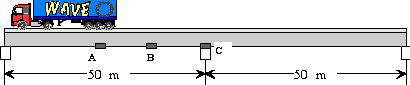
\includegraphics[width=12.277cm,height=2.566cm]{openwim-img/openwim-img3.pdf}
\par}

{\centering\selectlanguage{slovene}\bfseries
Figure 1 – This is a sample figure caption
\par}


\bigskip

{\selectlanguage{english}
All writing within figures should, where possible, be in 10.5-point
Times New Roman. Please note that color images will be printed in black
and white in the paper proceedings and must remain understandable. }

\subsection{Tables}
{\selectlanguage{english}
Table captions should be above the table, flush left, and in 11-point
Times New Roman. \ Separate table captions from body text and the table
with one line space above and below the captions as below. \ }


\bigskip

{\selectlanguage{english}\bfseries
Table 1 - Summary statistics for pre-weighed trucks (COV = Coefficient
of Variance)}


\bigskip

\begin{flushleft}
\tablehead{}
\begin{supertabular}{|m{2.799cm}|m{2.052cm}|m{2.0509999cm}|m{2.0509999cm}|m{2.0509999cm}|m{2.0509999cm}|m{1.7969999cm}|}
\hline
~
 &
\multicolumn{2}{m{4.3030005cm}|}{\centering \selectlanguage{english}
Type 1} &
\multicolumn{2}{m{4.302cm}|}{\centering \selectlanguage{english} Type 4}
&
\multicolumn{2}{m{4.0480003cm}|}{\centering \selectlanguage{english}
Type 5}\\\hline
~
 &
\centering \selectlanguage{english} Gross &
\centering \selectlanguage{english} Axle &
\centering \selectlanguage{english} Gross &
\centering \selectlanguage{english} Axle &
\centering \selectlanguage{english} Gross &
\centering\arraybslash \selectlanguage{english} Axle\\\hline
\selectlanguage{english} Mean IF &
\centering \selectlanguage{english} 1.00 &
\centering \selectlanguage{english} 0.98 &
\centering \selectlanguage{english} 1.03 &
\centering \selectlanguage{english} 1.03 &
\centering \selectlanguage{english} 1.02 &
\centering\arraybslash \selectlanguage{english} 1.02\\\hline
\selectlanguage{english} COV (\%) &
\centering \selectlanguage{english} 7.21 &
\centering \selectlanguage{english} 9.86 &
\centering \selectlanguage{english} 6.21 &
\centering \selectlanguage{english} 8.44 &
\centering \selectlanguage{english} 5.18 &
\centering\arraybslash \selectlanguage{english} 7.85\\\hline
\selectlanguage{english} Within 15\% &
\centering \selectlanguage{english} {}-{}-{}-{}-{}- &
\centering \selectlanguage{english} 93 &
\centering \selectlanguage{english} {}-{}-{}-{}-{}- &
\centering \selectlanguage{english} 94 &
\centering \selectlanguage{english} {}-{}-{}-{}-{}- &
\centering\arraybslash \selectlanguage{english} 85\\\hline
\end{supertabular}
\end{flushleft}

\bigskip

{\selectlanguage{english}
Tables should use 1-point lines for the top and bottom, and a half-point
line beneath the table’s header. \ Thickness of all table lines must be
0.5 point. All writing within tables should, where possible, be in
11-point Times New Roman. Cells’ content should be centered as much as
possible if relevant.}

\subsection{Equations and Units}
{\selectlanguage{english}
All equations should be indented 1.2 cm from the left margin and
numbered in brackets in the extreme right hand side of the page as
follows:}


\bigskip

{\selectlanguage{english}
\ \ \textit{C}\ \ =\ \ 
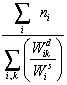
\includegraphics[width=2.011cm,height=2.54cm]{openwim-img/openwim-img4.pdf}
\ \ \ \ \ \ \ \ \ \ \ \ \ \ \ \ (2)}

\section{Electronic Submission Instructions}
{\selectlanguage{english}
Papers must be submitted by email (up to 6 Mb file size) or large file
transfer protocol to: \href{mailto:iswim@free.fr}{iswim@free.fr}, as
Microsoft Word files (.DOC or .DOCX) or RTF (Rich Text Format) files. }

{\selectlanguage{english}
You may use for example: \url{https://www.wetransfer.com} (but any other
file transfer web site may be used).}

\subsection{Word Files}
{\selectlanguage{english}
If you plan to include photographs or other images in your Microsoft
Word document, please use the “Insert” menu to place images in your
file rather than copying and pasting from another file. \ Do not link
to the image file.}

\subsection{Photographs}
{\selectlanguage{english}
Photographs should be set at a resolution of 300 dots per inch (dpi).
Photographs with lower resolution have much poorer print quality. Use
.JPG file with a rate of compression which maintains the file size of
each picture below app. 500 kbytes. Be careful to adjust the final size
of each picture in your photo editor, and import them as 1:1 scale in
the Word or RTF file (in order to prevent excessively large file
size).}


\bigskip

{\selectlanguage{english}
The photographs will be published in black and white in the paper
proceedings.}


\bigskip

{\selectlanguage{english}
A list of references should be given at the end of the paper. In the
body of the paper, references should be referred to by author and year.
For example: “Jones and Smith (1996) have extended the theory to
in-motion systems” or “Kellser’s theory for WIM systems (1995) has
shown” or “the theory for pseudo-static systems is well established
(Kessler, 1995).” }


\bigskip

{\selectlanguage{english}
The reference list style should be as follows (the first is a book, the
second and third are conference papers, and the last is a journal
paper):}

\section{References}
\liststyleWWNumvi
\begin{itemize}
\item {\selectlanguage{english}
Jones, J.M. (1992), Elements of WIM Systems in Operation, E \& F-N
Spon.}
\item {\selectlanguage{english}
O{\textquotesingle}Brien, E.J. and Sclob, J.M. (1993), \ “Prediction of
Extreme Load Effects in Highway Bridges”, in \textit{Proceedings of the
9}\textit{\textsuperscript{th}}\textit{ International Conference on
Highway Structures}, eds. A.M. O{\textquotesingle}Reilly and J.V.
Smith, Warsaw, Poland, 131-143.}
\item {\selectlanguage{english}
O{\textquotesingle}Connor, W.D., Bloggs, J. and Smith, J.J. (1994), “A
Proposed Renewable Energy Source”, in \textit{Proc. 2nd Int. Congress
on Innovation}, eds A.B. Jones and Smith, Elsevier Press, 2, 121-130.}
\item {\selectlanguage{english}
Freud, S.J., Smith, A.W. and Mannion, A.N. (1992), “A New Approach to
Behaviourism”, \textit{Journal of Structural Engineering}, Am. Soc.
Civ. Engnrs, 12, 1463-1479.}
\end{itemize}
{\centering\selectlanguage{english}\bfseries
\ FRONT PAGE FOR 3 AND 4 AUTHORS
\par}


\bigskip

\begin{flushleft}
\tablehead{}
\begin{supertabular}{m{3.8749998cm}m{3.8760002cm}m{3.8760002cm}m{3.8749998cm}}


\includegraphics[width=2.619cm,height=3.307cm]{openwim-img/openwim-img5.png}
 &


\includegraphics[width=2.619cm,height=3.307cm]{openwim-img/openwim-img6.png}
 &


\includegraphics[width=2.619cm,height=3.307cm]{openwim-img/openwim-img7.png}
 &


\includegraphics[width=2.619cm,height=3.307cm]{openwim-img/openwim-img8.png}
\\
\centering {\selectlanguage{english}\bfseries A. AUTHOR1}\par

\centering \selectlanguage{english} Organization 1\newline
Place 1 &
\centering {\selectlanguage{english}\bfseries B. AUTHOR2}\par

\centering \selectlanguage{english} Organization 2\newline
Place 2 &
\centering {\selectlanguage{english}\bfseries C. AUTHOR3}\par

\centering \selectlanguage{english} Organization 3\newline
Place 3 &
\centering {\selectlanguage{english}\bfseries D. AUTHOR4}\par

\centering\arraybslash \selectlanguage{english} Organization 4\newline
Place 4\\
\end{supertabular}
\end{flushleft}

\bigskip


\bigskip

{\selectlanguage{english}\bfseries
Abstract}

{\selectlanguage{english}
This paper gives instructions for the preparation of papers to be
presented at the 7\textsuperscript{th} International Conference on
Weigh-In-Motion (ICWIM7). It is presented, as far as is possible, in a
style consistent with a conference paper. Abstracts for these papers
should not exceed 10 lines in length. The abstract should be provided
in English and in one other language among French, Portuguese or
Spanish\footnote{ The French, Portuguese or Spanish version will be
edited if needed by a native speaking Scientific Committee member.}.
Nothing except the author details, photographs and abstracts should be
present on the first page.}


\bigskip

{\selectlanguage{english}
The papers will be first published in the conference proceedings, later
on the ISWIM website, and the best ones may be submitted to a Journal
with the authors’ agreement.}


\bigskip

{\selectlanguage{english}
\textstyletablecaptionCar{Keywords:} \ Language, Font, Photograph, Heavy
Vehicles, Freight transport, Weigh-in-Motion, WIM.}


\bigskip

{\selectlanguage{english}\bfseries
\foreignlanguage{french}{Résumé}}

{\selectlanguage{english}
\foreignlanguage{french}{Ce papier donne les instructions pour la
préparation des articles qui seront présentés à la
7}\foreignlanguage{french}{\textsuperscript{e}}\foreignlanguage{french}{
conférence internationale sur le pesage en marche (ICWIM7). Ces
instructions sont aussi proches que possible de celles de la plupart
des articles de conférences. Les résumés de ces articles ne doivent pas
dépasser 10 lignes. Le résumé doit être produit en anglais et dans une
autre langue à choisir parmi le français, l’espagnol ou le portugais.
Rien d’autre que les informations concernant les auteurs, leurs photos
et le résumé ne doit figurer sur la première page.}}


\bigskip

{\selectlanguage{english}
\foreignlanguage{french}{Les articles seront d’abord publiés dans les
actes de la conférence, puis sur le site ISWIM. Les meilleurs pourront
être soumis à une revue avec l’accord des auteurs.}}


\bigskip

{\selectlanguage{english}
\textstyletablecaptionCar{\foreignlanguage{french}{Mots-clés:}}\foreignlanguage{french}{
Langue, police, photos, poids lourds, transport de marchandises, pesage
en marche, WIM.}}


\bigskip
\end{document}
